\documentclass[11pt]{article}
\usepackage{fullpage}
\usepackage{graphicx}
\usepackage{tikz}
\usepackage{hyperref}

\title{CS63 Spring 2024\\Lab 6: Explaining XOR Network}
\author{Yana Yuan, Mavis Gao}

\begin{document}

\maketitle

With random seed 3
the XOR network achieved 100\% accuracy on the XOR data set after
1369
training epochs.  The resulting neural network is shown in the
following diagram.

\begin{center}
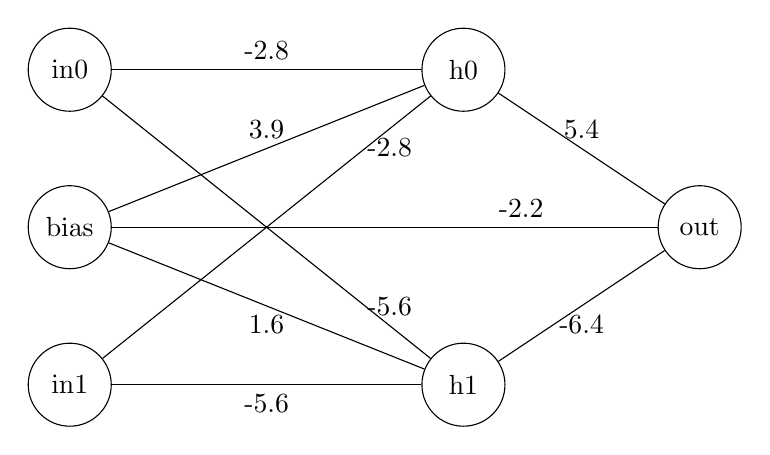
\begin{tikzpicture}
\tikzstyle{neuron}=[draw, circle, minimum size=30pt]

\draw (0,2) node[neuron] (bias) {bias};
\draw (0,4) node[neuron] (in0) {in0};
\draw (0,0) node[neuron] (in1) {in1};
\draw (5,4) node[neuron] (h0) {h0};
\draw (5,0) node[neuron] (h1) {h1};
\draw (8,2) node[neuron] (out) {out};

\draw (in0) edge node[above] {-2.8} (h0);
\draw (in0) edge node[very near end, above] {-5.6} (h1);
\draw (in1) edge node[very near end, below] {-2.8} (h0);
\draw (in1) edge node[below] {-5.6} (h1);
\draw (h0) edge node[above] {5.4} (out);
\draw (h1) edge node[below] {-6.4} (out);
\draw (bias) edge node[above] {3.9} (h0);
\draw (bias) edge node[below] {1.6} (h1);
\draw (bias) edge node[near end, above] {-2.2} (out);
\end{tikzpicture}
\end{center}

Based on these weights, this network solves XOR as follows.

A hidden node is active when the weighted sum of inputs exceeds the threshold 
that sigmoid function defines.
The weights in the network generally encourage inputs that are different and 
a larger output will therefore be generated to pass the threshold.

- for input (0,0): Both h0 and h1 would receive only the bias input making the
the weighted sum of h0 and h1 negative and further results in a sigmoid close to 0.
In this case, the output node only receives -2.2 from the bias node so the sigmoid is
again close to 0, which is correct for XOR. 

- for input (0,1): h0 would receive the bias node * 3.9 and -2.8 * in1
 as the in0 is 0, which is less negative value than before, and the evaluation 
 the function will output a number larger than 0.5, and h1 will receive 
 the bias node * 1.6 and -5.6 * in1, which the sum is a large negative number, 
 and the activation function will output the sigmoid close to 0; then the output
 the node receives a large positive value from h0 * the weight 5.4 and a small negative value
 bias * -2.2 and a small value h1 * -6.4, and since h1 sigmoid value is small, and that the sum
 of h0, bias, and h1 will be greater than 0.5 as the output node is influenced more
 by h0, which will result in an output close to 1, which is correct for XOR. 

- for input (1,0): the case is similar for (1, 0) compared to the case for (0, 1), 
where h0 will receive the bias node * 3.9 + -2.8 * in0 as in1 is 0, which is a positive value
and that the sigmoid will be larger than 0.5, and for h1, it receives -5.6 * in0 and 1.8 * bias node, 
which is a large negative number that will lead to the sigmoid being small and less than 0.5, and since
the output node receives 5.4 * h0 + -2.2 * weight and -6.4 * h1, and h0 has a higher sigmoid than h1, 
then the output would be close to 1 because the output node is influenced more by h0, which 
is correct for XOR. 

- for input (1,1): in this case, h0 receives in0 * -2.8 + bias * 3.9 + in1 * -2.8, which is a 
negative number and have the sigmoid close to 0, and for h1, h1 receives in0 * -5.6 + bias * 1.6 + in1 * -5.6, 
which is a large negative number and has the sigmoid to be close to 0, in this case, 
the output is influenced more on the -2.2 * bias node which is a negative value as well so the sigmoid is close to 0, 
which is correct for XOR. 
 

\end{document}
